La fusione nucleare è di fatto la sorgente di energia che alimenta il sole. Qui verrà trattato il processo in maniera un po' più quantitativa. I fenomenti che determinano il tasso della reazione \textbf{picco di Gamow} e energia irraggiata e "durata" del sole.
\subsection{Reazioni nucleari nel sole}
%IMMAGINE rea
\begin{figure}[htp!]
  \centering
  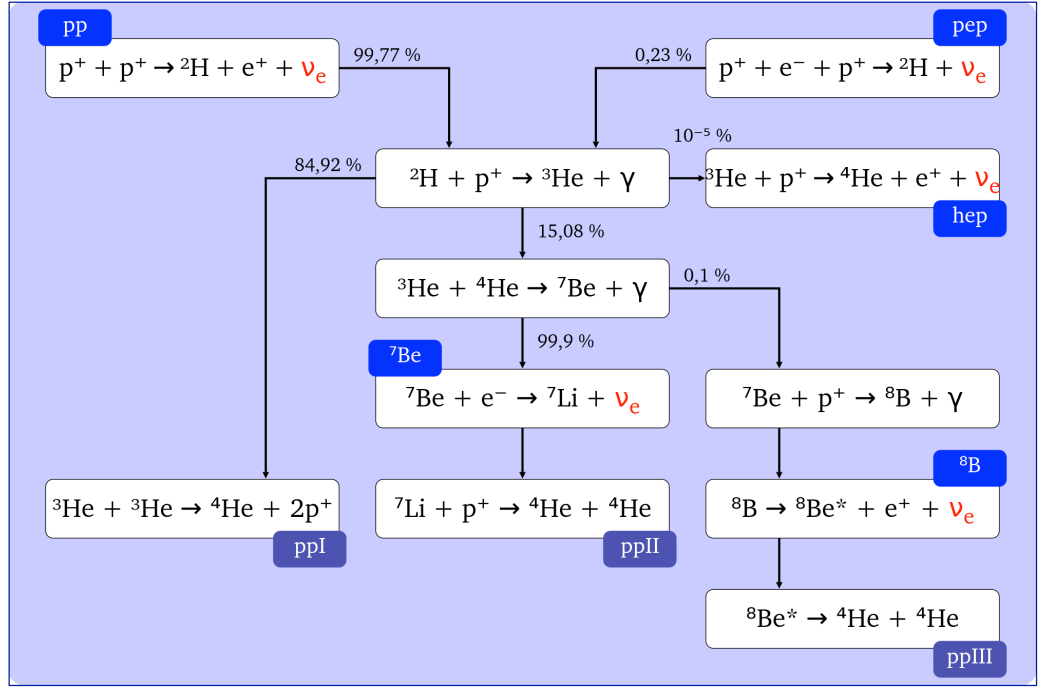
\includegraphics[scale=0.35]{Lezione10/rea.png} 
\end{figure}
Queste reazioni nucleari partono principalmente, quasi sempre, con delle interazioni deboli che sono simili a dei decadimenti $\beta$ non lo sono perchè sono abbinate delle fusioni ma comunque trasformazioni in protoni e neutroni in cui viene liberata energia. Oltre a questo si nota come ci sia una sorta di catena principale in cui la maggior parte dell'energia viene prodotta in questo modo. Questa sequenza di fusione principale è data dalle reazioni:
\begin{equation*}
    \ch{^1H}+  \ch{^1H}\to   \ch{^2H}+e^++\nu_e \qquad +0.42\,MeV
\end{equation*}
il passo successivo è che questo deutone si mangia un altro protone e diventa elio-3:
\begin{equation*}
    \ch{^2H}+\ch{^1H}\to \ch{^3He}+\gamma \qquad +5.49\,MeV
\end{equation*}
Quello che succede poi gli atomi di elio-3 possono fondersi per produrre un elio-4 con l'espulsione di due protoni in eccesso che possono ritornare in cima alla catena:
\begin{equation*}
    \ch{^3He}+\ch{^3He}\to\ch{^4He}+2\ch{^1H} \qquad +12.86\,MeV
\end{equation*}
Per quanto riguarda i guadagni energetici per la prima reazione abbiamo abbiamo:
\begin{align*}
    Q=2m( \ch{^1H})\,\,\,\,2u+14.58\,MeV \\
    -m( \ch{^2H})\,\,\,\,-2u-13.14\,MeV \\ 
    -2m_e \,\,\,\,\,\,\,\,\,\,\,\,-1.02\,MeV \\
    =0.42\,MeV
\end{align*}
Per la seconda abbiamo:
\begin{align*}
    Q=m( \ch{^2H})\,\,\,\,2u+13.13\,MeV \\
    +m( \ch{^1H})\,\,\,\,1u+7.29\,MeV \\ 
    -m(\ch{^3He})\,\,\,\,-3u -14.93\,MeV \\
    =5.49\,MeV
\end{align*}
E per la terza reazione:
\begin{align*}
    Q=2m( \ch{^3He})\,\,\,\,6u+29.86\,MeV \\
    -m( \ch{^4H})\,\,\,\,-4u-2.42\,MeV \\ 
    -2m(\ch{^1H})\,\,\,\,-2u -14.58\,MeV \\
    =12.86\,MeV
\end{align*}
Il grosso dell'energia viene prodotta dai processi in cui entrano le interazioni forti. Ma questo processo è nato da un processo di interazione debole che porta poca energia ma è il passo fondamentale che ci da i neutroni. Infatti il nuetrone da solo non può esistere ed ha un tempo di decadimento di circa 15 minuti. Grazie al processo di fusione del primo processo porta alla formazione di un neutrone fondamentale per dopo. Il risultato netto di 2 volte le prime due reazioni porta alla terza:
\begin{equation*}
    6(\ch{^1H})\to \ch{^4He}+2(\ch{^1H})+2e^++2\nu_e+2\gamma+24.68\,MeV
\end{equation*}
E quindi:
\begin{equation*}
      4(\ch{^1H})\to \ch{^4He}+2e^++2\nu_e+2\gamma+24.68\,MeV
\end{equation*}
Questa è la reazione principale che dobbiamo tenere a mente: quattro protoni si fondono a dare un nucleo di elio e in questo processo c'è la produzione di neutrini positroni e un rilascio di energia. 

Nuclei più pesanti dell'elio posso formarli dalla fusione di questi nuclei di elio prodotti precedentemente. Infatti nuclei pesanti possono venire prodotti dalla fusione di particelle $\alpha$:
\begin{equation*}
    3(\ch{^4He})\to \ch{^{12}C}+7.27\,MeV
\end{equation*}
Questo permette altre catene, ad esempio la sequenza del ciclo CNO (carbonio azoto ossigeno):
\begin{align*}
      ^{12} \mathrm{C}+{ }^1 \mathrm{H} \rightarrow{ }^{13} \mathrm{~N}+\gamma & +1.95 \mathrm{MeV} \\ { }^{13} \mathrm{~N} \rightarrow{ }^{13} \mathrm{C}+e^{+}+v_e & +1.20 \mathrm{MeV} \\ { }^{13} \mathrm{C}+{ }^1 \mathrm{H} \rightarrow{ }^{14} \mathrm{~N}+\gamma & +7.55 \mathrm{MeV} \\ { }^{14} \mathrm{~N}+{ }^1 \mathrm{H} \rightarrow{ }^{15} \mathrm{O}+\gamma & +7.34 \mathrm{MeV} \\ { }^{15} \mathrm{O} \rightarrow{ }^{15} \mathrm{~N}+e^{+}+v_e & +1.68 \mathrm{MeV} \\ { }^{15} \mathrm{~N}+{ }^1 \mathrm{H} \rightarrow{ }^{12} \mathrm{C}+{ }^4 \mathrm{He} & +4.96 \mathrm{MeV}
\end{align*}
Il $\ch{^{12}C}$ funge come una sorta di catalizzatore, e l'effetto netto è sempre:
\begin{equation*}
     4(\ch{^1H})\to \ch{^4He}+2e^++2\nu_e+2\gamma+24.68\,MeV
\end{equation*}
Infatti se guardo la catena precedente tanto carbonio avevo all'inizio me lo trovo alla fine, ciò che produco lo consumo e quindi l'effetto netto è che quello che prendo come combustibile è l'idrogeno.
\subsection{La vita del sole}
Il sole ha una massa $M=2\times10^{30}\,kg$, costituiti in massima parte da idrogeno. Gli atomi di idrogeno presenti sono: $N_H=MN_A/A=1.2\times10^{57}$. La potenza irraggiata dal sole è $L=4\times10^{36}\,W$. Il numero di cicli di fusione al secondo: $L/24.69\,MeV$. Ogni ciclo di fusione brucia $4$ atomi di idrogeno:
\begin{equation*}
    \frac{dN_H}{dt}=4\frac{L}{24.68\,MeV}=4\times10^{38}s^{-1}
\end{equation*}
cioè ogni secondo brucio questi atomi di idrogeno. Il combustibile si esaurisce in un tempo:
\begin{equation*}
    T=\frac{N_H}{dN_H/dt}=0.3\times10^{19}\,s
\end{equation*}
Che equivale a circa $100$ miliardi di anni. La terra ha circa $5$ miliardi di anni, quindi sappiamo che effettivamente la fusione è una sorgente di energia molto efficace che permette la sopravvivenza delle stelle per così tanto tempo. Prima della relatività ristretta si supponeva che l'energia prodotta dal sole fosse di origine gravitazionale. Visto che all'epoca c'erano solo due forze fondamentali. La gravità e quella elettromagnetica.
\subsection{Barrirera Coulombiana}
Perchè una reazione tra nucleo $X$ ed il nucleo $Y$ possa avvenire bisogna superare la barriera coulombiana. Banalmente per fondere due nuclei devo mettere molta energia perchè tenderebbero a respingersi.
\begin{equation*}
    V=\frac{e^2}{4\pi\varepsilon_0}\frac{Z_XZ_Y}{R_Z+R_Y}=\frac{e^2}{4\pi\varepsilon_0\hbar c}\frac{\hbar c}{R_Z+R_Y}Z_XZ_Y=\alpha\frac{\hbar c}{R_Z+R_Y}Z_XZ_Y
\end{equation*}
Per la prima reazione della catena, $p+p$, $R_P\sim0.85\,fm$:
\begin{equation*}
    V_{pp}=\alpha\frac{\hbar c}{2R_p}=0.85\,MeV
\end{equation*}
Il problema è quanti di questi protoni nel sole hanno l'energia sufficiente per superare tale barriera: i protoni, ad una temperatura $T$ avranno una distribuzione di velocità alla Maxwell-Boltzmnann:
\begin{equation*}
    \frac{dN}{dv}=N\sqrt{\frac{2}{\pi}}\left(\frac{m_p}{kT}\right)^{3/2}v^2\text{exp}\left(-\frac{1}{2}\frac{m_pv^2}{kT}\right)
\end{equation*} 
In realtà non è così! Trasformiamola in termini di energia cinetica:
\begin{equation*}
     \frac{d N}{d E}=\frac{d N}{d v} \frac{d v}{d E}=N \sqrt{\frac{2}{\pi}}\left(\frac{m_p}{k T}\right)^{3 / 2} \frac{2 E}{m_p} \exp \left(-\frac{E}{k T}\right) \frac{1}{\sqrt{2 m_p E}}=N \frac{2}{\sqrt{\pi}}\left(\frac{1}{k T}\right)^{3 / 2} \sqrt{E} \exp \left(-\frac{E}{k T}\right)
\end{equation*}
Dove abbiamo usato:
\begin{equation*}
   E=\frac{1}{2} m_p v^2 \quad v=\sqrt{2 E / m_p} \quad \frac{d v}{d E}=\sqrt{\frac{2}{m_p}} \frac{1}{2} \frac{1}{\sqrt{E}}=\frac{1}{\sqrt{2 m_p E}}
\end{equation*}
La frazione di protoni con $E>V_{pp}$ (mettendo $x=\frac{E}{k T}$)
\begin{align*}
f  =\frac{1}{N} \int_{V p p}^{+\infty} d E \frac{d N}{d E}=\int_{V p p}^{+\infty} d E \frac{2}{\sqrt{\pi}}\left(\frac{1}{k T}\right)^{3 / 2} \sqrt{E} \exp \left(-\frac{E}{k T}\right)=\frac{2}{\sqrt{\pi}} \int_{V_{p p} / k T}^{+\infty} d x \sqrt{x} \exp (-x) \quad \\  =\left[\operatorname{erf}(\sqrt{x})-\frac{2}{\sqrt{\pi}} \sqrt{x} \exp (-x)\right]_{V_{p p} / k T}^{+\infty}=1-\operatorname{erf}\left(\sqrt{\frac{V_{p p}}{k T}}\right)+\frac{2}{\sqrt{\pi}} \sqrt{\frac{V_{p p}}{k T}} \exp \left(-\frac{V_{p p}}{k T}\right) 
\end{align*}
con 
\begin{equation*}
\operatorname{erf}(x)=\frac{2}{\sqrt{\pi}} \int_0^x d x e^{-\frac{1}{2} x^2}
\end{equation*}
Al centro del sole $T\sim15\times 10^{6}\,K$, $kT$. Usando l'espressione approssimata degli essori 
\begin{align*}
    1-\operatorname{erf}(x) \stackrel{x \rightarrow+\infty}{\longrightarrow} \exp \left(-x^2\right) / \sqrt{\pi} x \\ f=\left[\frac{1}{\sqrt{\pi}}\left(2 \sqrt{\frac{V_{p p}}{k T}}+\sqrt{\frac{k T}{V_{p p}}}\right) \exp \left(-\frac{V_{p p}}{k T}\right)\right]
\end{align*} 
Per vedere immediatamente l'ordine di grandezza, estraiamo il logaritmo:
\begin{equation*}
  \log _{10} f=\log _{10}\left[\frac{1}{\sqrt{\pi}}\left(2 \sqrt{\frac{V_{p p}}{k T}}+\sqrt{\frac{k T}{V_{p p}}}\right) \exp \left(-\frac{V_{p p}}{k T}\right)\right]=1.5-\frac{V_{p p}}{k T} \log _{10} e=-282.5
\end{equation*}
Quindi la frazione di protoni che ha energia sufficiente per superare la barriera di potenziale è $10^{-282}$. Abbiamo $10^{57}$ protoni, quindi i protoni che hanno energia a sufficienza per superare la barriera sono praticamente nulli. Quindi la risposta risiede nell'effetto tunnel.
\subsection{Picco di Gamow}
\textbf{Reazioni di fusione} alle \textbf{temperature stellari} sono possibili solo grazie all'attraversamento della barriera Coulombiana per \textbf{effetto tunnel}. Lo stesso fattore di Gamow che entra nel decadimento $\alpha$:
\begin{equation*}
    G=\sqrt{\frac{2m_p}{\hbar^2 E}}\frac{e^2}{4\pi\varepsilon_0}f\left(\frac{2R_p}{b}\right)
\end{equation*}
La sezione d'urto effettiva:
\begin{equation*}
    \sigma(E)=e^{-2G}\sigma_0(E)
\end{equation*}
dove $\sigma_0$ rappresenta la sezione d'urto in assenza di repulsione coulombiana. Quindi la probabilità di interazione $\lambda$ per un protone di energia $E$ è data da:
\begin{equation*}
    \lambda=v\sigma(E)n_p
\end{equation*}
Questa ha come unità di misura l'inverso del tempo ed è la probabilità per unità di tempo per un protone di fare fusione. $n_p$ è la densità di protoni. Il tasso di interazioni per unità di volume ad una certa energia:
\begin{equation*}
    \frac{dn_{int}}{dt}(E)=n_p(E)\sqrt{\frac{2E}{m_p}}e^{-2G(E)}\sigma_0(E)n_p
\end{equation*}
%IMMAGINE ty
\begin{figure}[htp!]
  \centering
  
\includegraphics[scale=0.8]{Lezione10/ty.png} 
\end{figure}
Qui abbiamo che il tasso di interazioni per unità di energia contiene due fattori: uno è il numero di protoni per una certa energia che contiene il fattore $e^{-E/kT}$ quindi è un numero grande per energie basse e tende a diminuire per alte energie. Poi c'è il fattore di Gamow che ha un comportamento inverso. Il tasso di interazione avviene quindi preferibilmente ad una energia ben precisa. Detto il picco di Gamow.
\subsection{Reattività}
Il tasso di interazione ad una certa energia è dato da:
\begin{equation*}
     \frac{dn_{int}}{dt}(E)=n_p(E)\sqrt{\frac{2E}{m_p}}e^{-2G(E)}\sigma_0(E)n_p=n_p\frac{n_p(E)}{n_p}v(E)e^{-2G(E)}\sigma_0(E)n_p
\end{equation*}
Il tasso totale di interazioni per unità di volume:
\begin{equation*}
    \frac{dn_{int}}{dt}=n_p^2\int_0^{\infty}dE\frac{n_p(E)}{n_p}v(E)e^{-2G(E)}\sigma_0(E)
\end{equation*}
In generale per diverse specie: $\frac{dn_{int}}{dt}=n_Xn_Y\langle\sigma v\rangle$
Il prodotto $\langle\sigma v\rangle$ prende il nome di \textbf{reattività} e determina il tasso di interazione e dipende dalla temperatura del sistema. Il processo di fusione nel sole inizia con un'interazione debole e con una piccola sezione d'urto (che viene compensata dall'altissima densità di protoni che abbiamo a disposizione e dal volume):
\begin{equation*}
    \sigma\approx10^{-44}\,cm^2
\end{equation*}
Ora, perchè non posso usare la fusione nucleare per produrre energia? Il problema è che per produrre artificialmente energia non possiamo competere nè con l'energia nè con il volume del sole. Dobbiamo cercare qualcosa che abbia una reattività più alta. Devo partire da stati con già i neutroni che mi servono perchè devo per forza partire da interazioni forti. L'altra cosa è che cerco di andare a temperature più alte per aumentare la velocità media.
processi di fusione artificiale necessitano di avere tassi di maggiori interazione maggiori.
\subsection{Neutrini solari}
Il sole produce energia sintetizzando elementi pesanti partendo da elementi leggeri mediante un processo di fusione nucleare. La reazione di partenza è la produzione di deuterio partendo da nuclei di idrogeno
\begin{equation*}
    p+p\to d+e^++\nu_e
\end{equation*}
La rivelazione del neutrino avviene con un processo analogo a quello utilizzato per l'antineutrino
\begin{equation*}
    \nu_e+n\to p+e^-
\end{equation*}
Di fatto facciamo il processo inverso della rivelazione del neutrino nel decadimento $\beta$. La prima rivelazione del neutrino solare fu fatta da R. Davis negli anni $'60$ utilizzando un medoto radiochimico. L'interazione di $\ch{^{37}Ar}$ è radioattivo e decate con un tempo di dimezzamento di circa $35$ giorni. Il positrone ha un'energia massima di circa $800\,keV$.
\begin{equation*}
    \ch{^{37}Ar}\to\ch{^{37}Cl}+e^++\nu_e
\end{equation*}
Ricapitolando abbiamo visto i decadimenti $\beta$ e la fusione nucleare in cui è un processo a prima vista un'interazione forte ma uno dei passi fondamentali nelle stelle è proprio un processo debole che possiamo evidenziare proprio guardando i neutrini prodotti nella reazione. Nel sole questo processo va bene perchè abbiamo un volume gigantesco al fronte di una sezione d'urto bassa, riusciamo comunque ad avere un rate abbastanza alto.